\begin{minipage}[c][\textheight][c]{\linewidth}
    \section{Introducción}
    El presente documento tiene como objetivo presentar un algoritmo genético diseñado para abordar una problemática común en el ámbito estudiantil: la selección óptima de materias para un estudiante en un estado de irregularidad académica. Esta herramienta de software propone una solución que determina la distribución más adecuada de materias teniendo en cuenta las preferencias del estudiante, así como la secuencia recomendada dentro del plan de estudios y el progreso académico del mismo. La exposición detallada del análisis, la metodología empleada y el desarrollo del software facilita la comprensión de su funcionamiento y su aplicación práctica en el contexto educativo.
\end{minipage}

\newpage


\section{Análisis del Problema}
Para abordar la resolución de la problemática planteada, se llevó a cabo una exhaustiva identificación de los elementos pertinentes que influyen en el funcionamiento del algoritmo, así como su efectiva traducción para su implementación en un algoritmo genético.

\subsection{Problemática}
El núcleo del problema radica en la necesidad de planificar el horario académico del próximo cuatrimestre para un estudiante, basándose en su historial académico, el cual comprende un conjunto de materias que ha cursado o reprobado. Este desafío implica la evaluación de cada materia según su importancia relativa, el respeto a las preferencias del estudiante y la evitación de solapamientos de horarios entre las asignaturas. El funcionamiento general del algoritmo puede esquematizarse de la siguiente manera:

\begin{figure}[h]
    \centering
    % Se establece que ocupe el 100% del ancho del margen de texto
    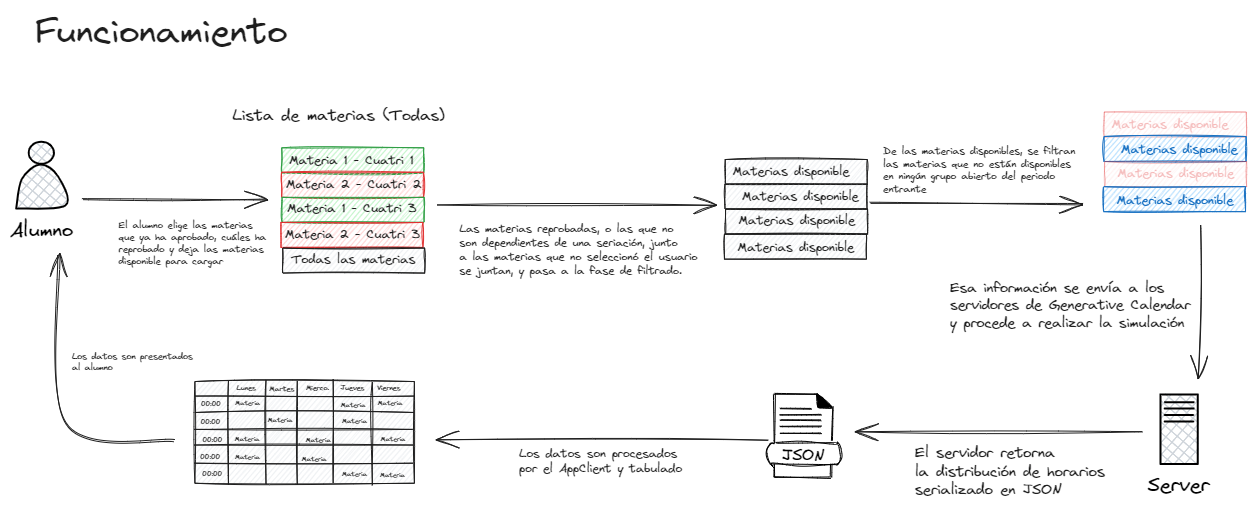
\includegraphics[width=\textwidth]{images/AG-funcionamiento.png}
    \label{Diagrama del funcionamiento general del algoritmo.}
    \caption{Diagrama del funcionamiento general del algoritmo.}
\end{figure}

\section{Resolución de problemas}
En esta sección se describe el enfoque adoptado para abordar el problema y alcanzar los objetivos del programa. La resolución del problema se divide en los siguientes puntos, que se detallarán a través de las diferentes subsecciones del documento.

\begin{enumerate}
    \item Captura de materias. $_{\text{\ref{captura_de_materias}}}$
    \item Filtrado de materias. $_{\text{\ref{filtrado_de_materias}}}$
    \item Cuantificación de los datos. $_{\text{\ref{cuantifiacion_de_datos}}}$
    \item Procesamiento de la información. $_{\text{\ref{procesamiento_de_la_informacion}}}$
\end{enumerate}

\subsection{Captura de materias} \label{captura_de_materias}
La primera etapa del proceso del algoritmo se centra en la captura de las materias cursadas por el alumno, lo que refleja su estado académico actual. En esta fase, el alumno seleccionará manualmente las materias que ha aprobado y las que ha reprobado, dejando libres aquellas que aún no ha cursado. Esta acción proporciona al sistema un contexto claro sobre el estado y el progreso del usuario. Además, la implementación de la seriación de materias, tema que se abordará en la siguiente sección, facilitará el completado y filtrado de las materias. %\\

\begin{figure}[h]
    \centering
    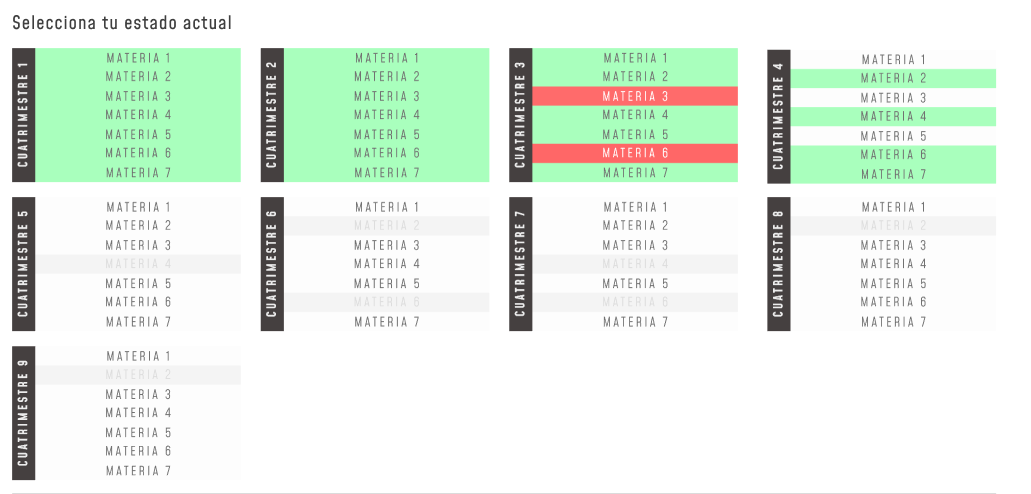
\includegraphics[width=\textwidth]{images/current_status_figma_screenshot.png}
    \caption{Captura de pantalla de la sección de selección de materias cursadas, obtenida del maquetado en Figma.}
    \label{fig:captura_materias}
\end{figure}


\subsection{Filtrado de materias} \label{filtrado_de_materias}
El proceso de filtrado de materias tiene como objetivo eliminar aquellas materias que, debido a restricciones de seriación, no deben considerarse al generar el nuevo horario académico. Estas materias, denominadas "posibles materias de carga", son aquellas que el algoritmo debe tomar en cuenta al generar el horario. Es importante destacar que el Algoritmo Genético (AG) procesa únicamente las posibles combinaciones de materias, sin validar directamente la existencia de dependencias entre ellas. %\\

Una vez que el usuario ha seleccionado las materias aprobadas, estas se guardan en un arreglo de materias \( M \), donde se almacenan todas las materias iniciales \( N \) etiquetadas según la selección del alumno. De esta forma, \( M \) se define como: %\\

\begin{equation}
    M : \{ N_1, N_2, \dots, N_i \}
    \label{eq:arreglo_materias_sin_procesar}
\end{equation} \myequations{Arreglo de materias sin procesar.}

\noindent
Donde \( N_i \) es la materia alojada en la posición \( i \) del arreglo \( M \), y se podría definir a \( N_i \) de la siguiente manera: %\\

\begin{equation}
    N_i : (\text{id}_i, \text{status}_i, [\text{dependencias}]_i, [\text{dependientes}]_i, \text{cuatrimestre}_i)
    \label{eq:atributos_materia}
\end{equation} \myequations{Atributos de las asignaturas sin procesar.}

\noindent
Donde cada atributo de los objetos materia obedece las siguientes definiciones:
\begin{itemize}
    \item \( \text{id} \): es el identificador único de la materia conformado por caracteres alfabéticos de longitud 4.
    \item \( \text{status} \): es el estado que ha elegido el alumno, que puede ser: aprobado, reprobado, o sin cursar.
    \item \( [\text{dependencias}] \): es un arreglo de longitud \( n \) que contiene todos los identificadores de las materias que se deben cursar antes de poder cursar la materia actual.
    \item \( [\text{dependientes}] \): es un arreglo de todas las materias que dependen de la materia actual, es decir, aquellas materias que se podrán cursar una vez que la materia actual haya sido aprobada.
    \item \( \text{cuatrimestre} \): corresponde a un identificador numérico del 1 al 9, que indica el cuatrimestre regular en el que debería ser cursada dicha materia.
\end{itemize}


\subsubsection{Seriación}
Es importante destacar que las materias contienen arreglos internos que hacen referencia a las materias dependientes y las materias dependencias. Esta característica se debe a la seriación, la cual dicta qué materias se podrán cursar en función del progreso del alumno. %\\

La seriación, comúnmente conocida, se ajusta al mapa curricular de la carrera para la cual se desarrolló el algoritmo. En el caso actual, dicho mapa curricular corresponde a la carrera de \textbf{Ingeniería en Desarrollo de Software} (IDS). %\\

El algoritmo se basó en el mapa curricular de IDS del año 2017. Como se puede observar en la figura \ref{fig:mapa_curricular_ids_2017}, existen materias que solo se podrán cursar una vez que todas las materias requeridas sean aprobadas. %\\

\begin{figure}[h]
    \centering
    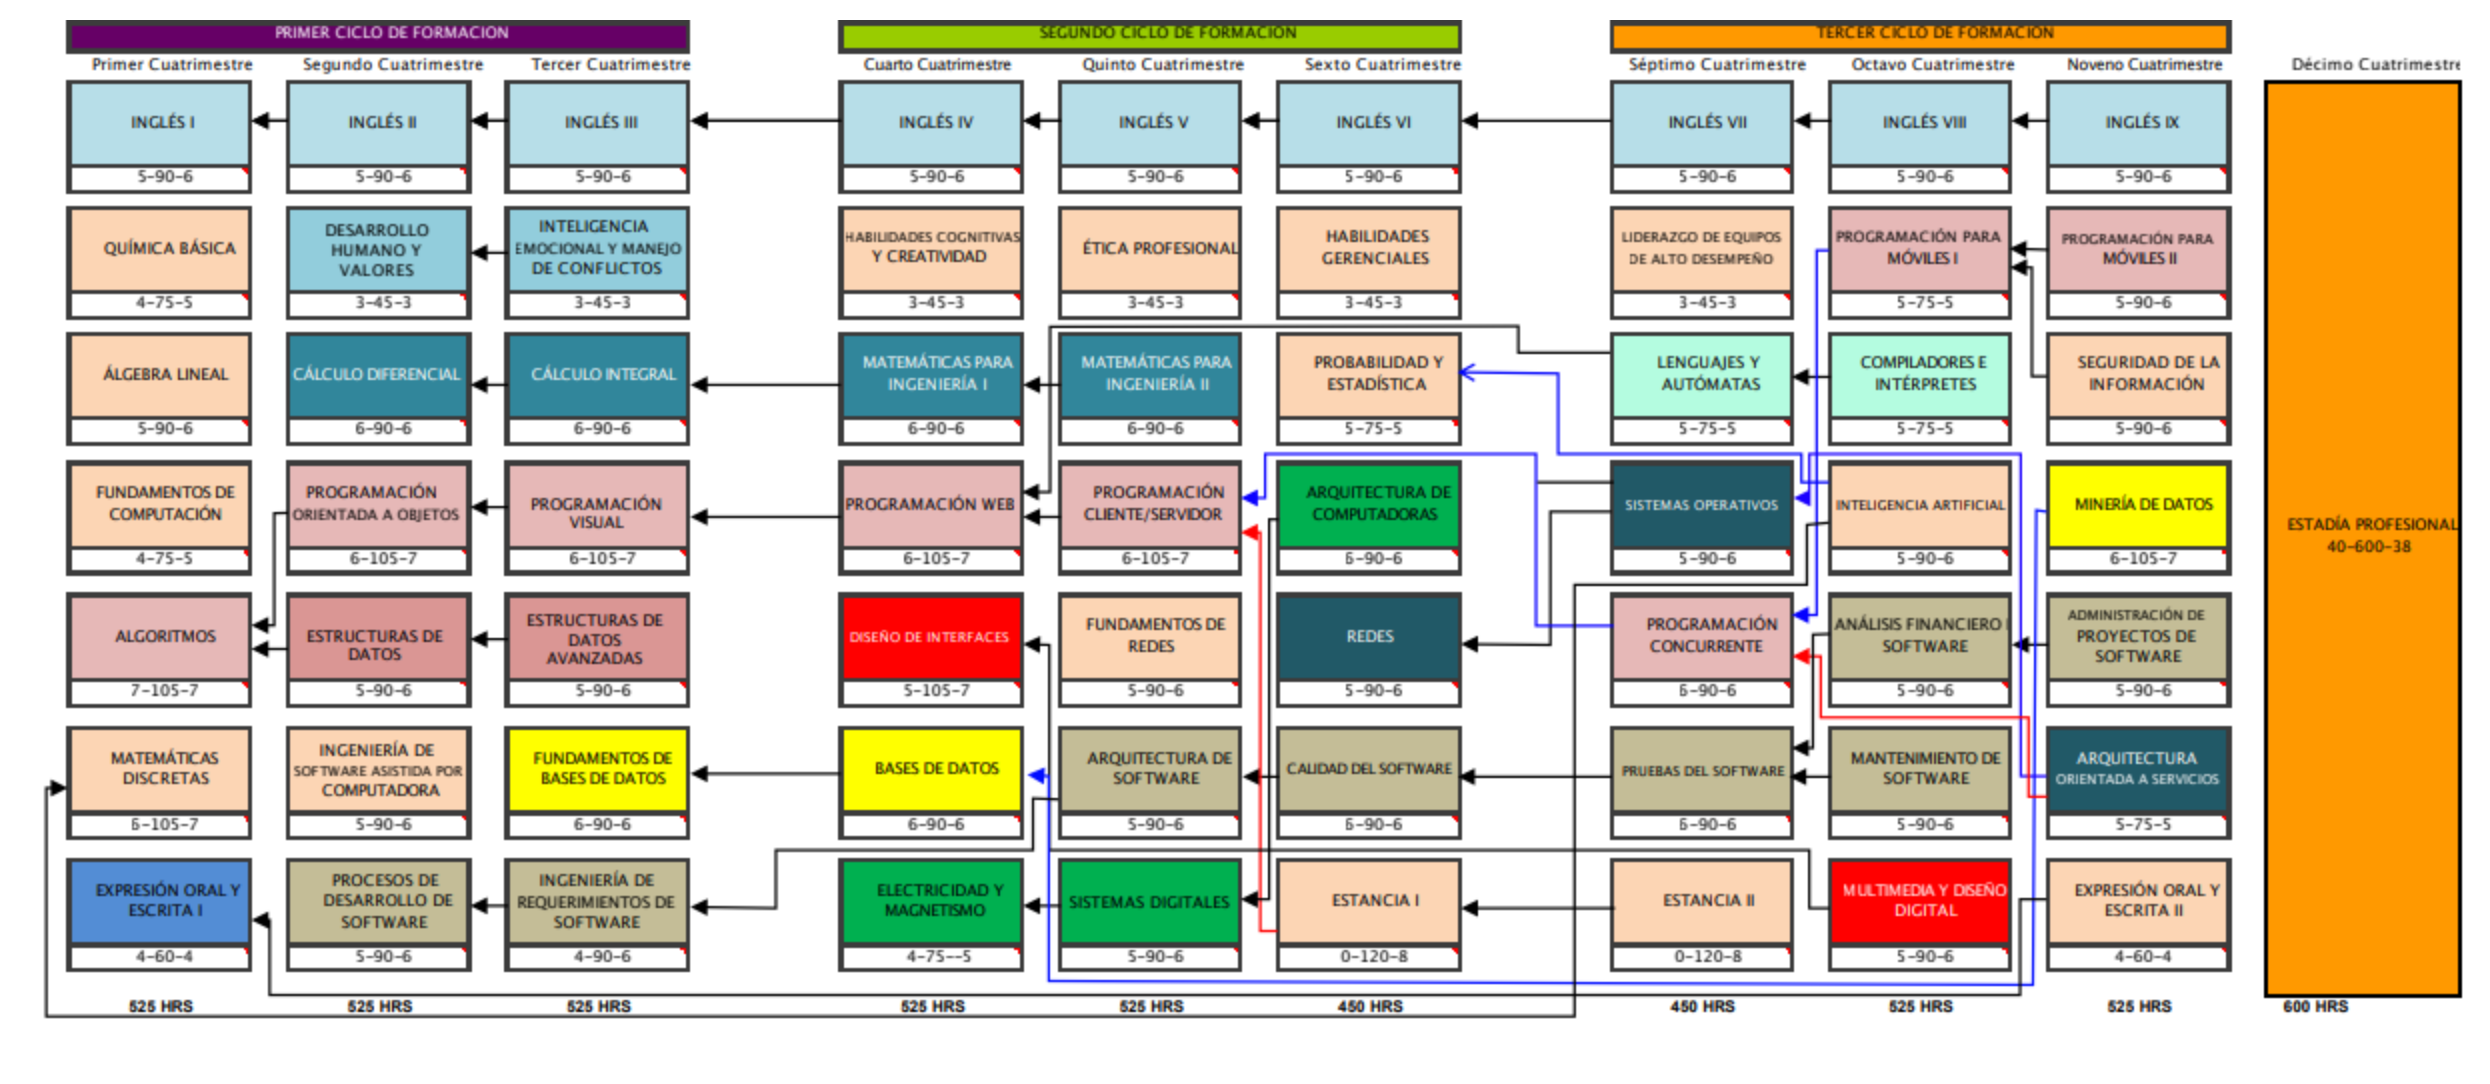
\includegraphics[width=\textwidth]{images/mapa_curricular.png}
    \caption{Mapa curricular de la carrera de Ingeniería en Desarrollo de Software del año 2017.}
    \label{fig:mapa_curricular_ids_2017}
\end{figure}


\subsubsection{Delimitación de materias} \label{delmitacion_de_materias}
Es fundamental tener en cuenta que existen materias que no pueden ser cursadas hasta que se aprueben una o más asignaturas de su línea de seriación. Por lo tanto, el programa debe eliminar de la lista de materias todas aquellas asignaturas que, según el caso de cada alumno, no sean aptas para ser cargadas debido a motivos de reprobación o porque su esquema de seriación está incompleto. %\\

Para ilustrar este concepto, consideremos un ejemplo y simplifiquemos el mapa curricular de la siguiente manera: %\\

\begin{figure}[h]
    \centering
    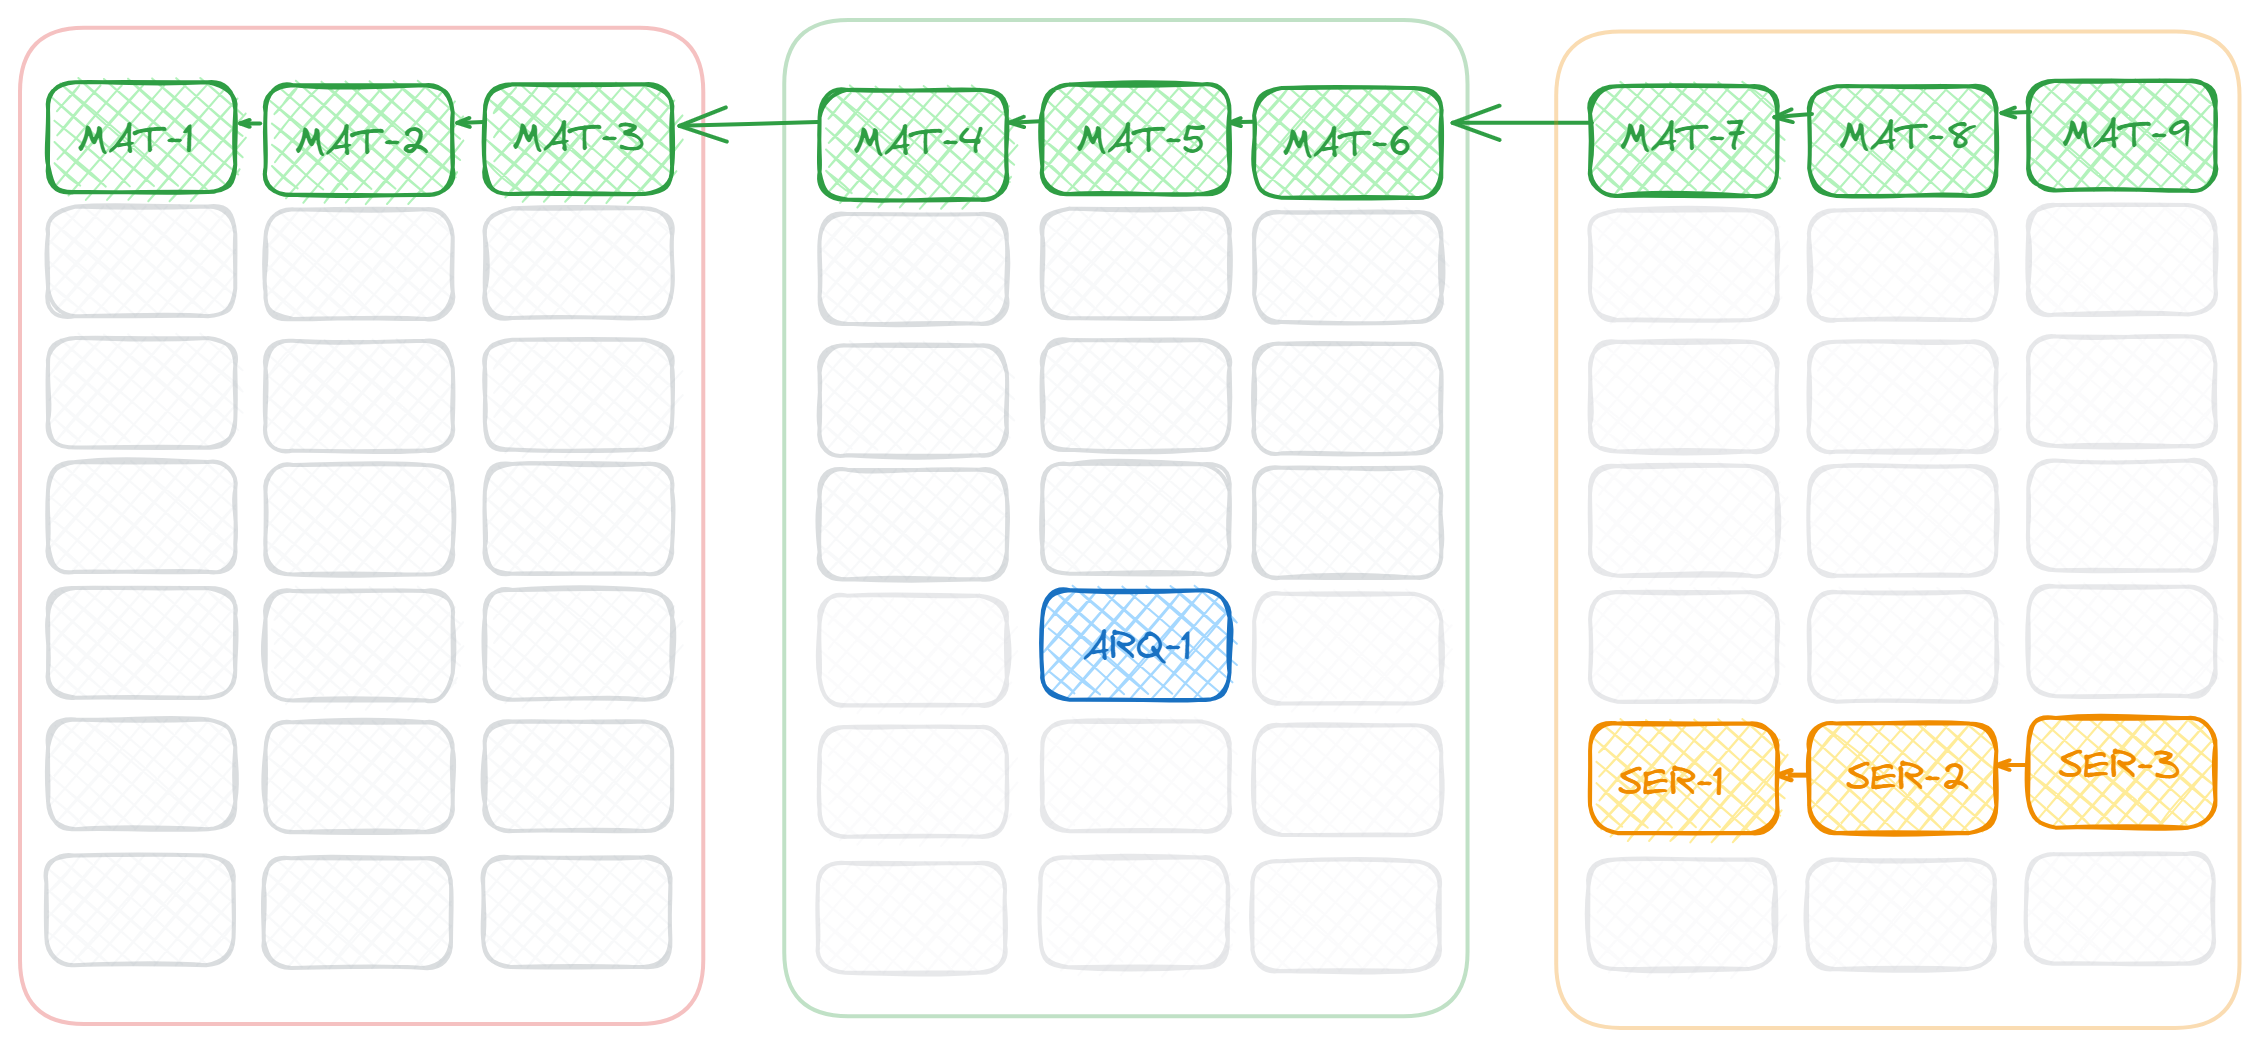
\includegraphics[width=0.8\textwidth]{images/AG-Simple-Serial-Squeme.png}
    \caption{Mapa curricular simplificado de ejemplo: Caso 1.}
    \label{fig:mapa_curricular_simplificado_caso_1}
\end{figure}

Teniendo un mapa curricular como el de la figura \ref{fig:mapa_curricular_simplificado_caso_1}, cada materia tiene una lista de asignaturas que dependen de ella. Por ejemplo: %\\
\begin{itemize}
    \item MAT-7 tiene una lista de materias dependientes donde se hallan MAT-8 y MAT-9.
    \item MAT-6 tiene una lista de materias dependientes donde se hallan MAT-7, MAT-8 y MAT-9.
\end{itemize}

Cuando una materia, por ejemplo ARQ-1, no tiene ninguna asignatura en su conjunto de materias dependientes, se le considera una materia débilmente seriada. Esto significa que ARQ-1 puede ser cursada sin tener ninguna otra materia como requisito previo. En otras palabras, no existen restricciones de seriación que limiten la capacidad de cursar ARQ-1 en función de otras asignaturas.

Ahora, si una materia es marcada como 'reprobada', todas las materias pertenecientes a la lista de materias dependientes de esa materia reprobada se marcarán como "deshabilitadas". Este proceso se aplica recursivamente a todas las materias dependientes de las materias deshabilitadas. Es decir, si una materia directamente dependiente de la materia reprobada se deshabilita, entonces todas las materias que dependen de esa materia también se deshabilitarán. La materia originalmente marcada como reprobada, sin embargo, será apta para volver a cargarse en futuros intentos académicos.

\clearpage

\begin{figure}[h]
    \centering
    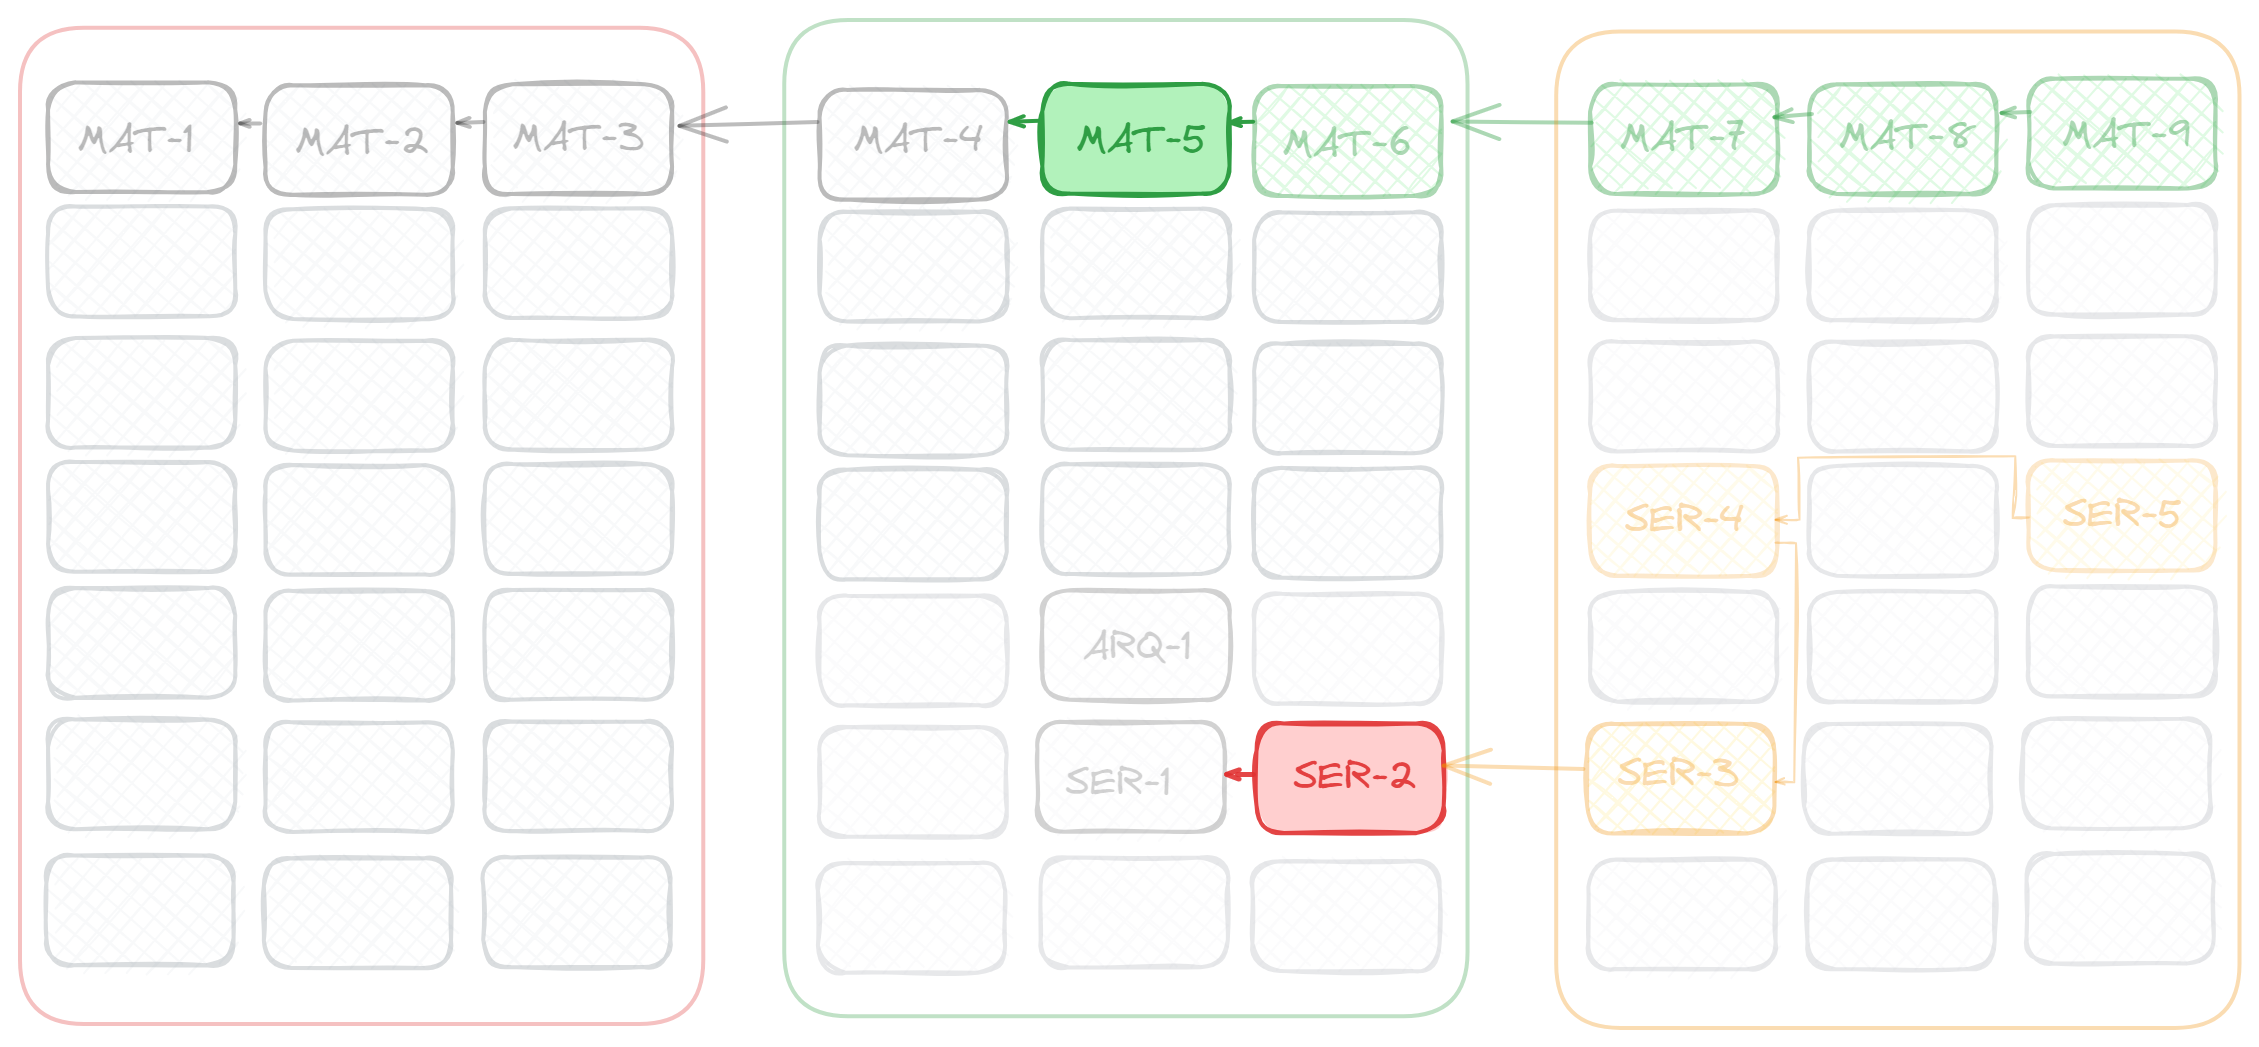
\includegraphics[width=0.8\textwidth]{images/AG-Simple-Serial-Squeme-2.png}
    \caption{Mapa curricular simplificado de ejemplo: Caso 2.}
    \label{fig:mapa_curricular_simplificado_caso_2}
\end{figure}
    
De manera similar, si una materia es seleccionada por el usuario y se encuentra dentro de al menos un conjunto de materias marcadas como reprobadas o no cursadas, esta materia también será marcada como "deshabilitada". Este proceso garantiza que no se programen materias que tengan dependencias no cumplidas o que hayan sido reprobadas previamente, garantizando así la coherencia del horario académico del estudiante.

Esta delimitación se realiza mediante una serie de condiciones algebraicas que describen el proceso de manera precisa.

Se define \( M \) como una materia, \( R \) como una materia marcada como reprobada o no cursada, \( P \) como el conjunto de materias con posibilidad de carga, y \( N \) como el conjunto de materias sin posibilidad de carga.

Entonces, estas condiciones pueden expresarse de la siguiente manera:

\begin{itemize}
    \item Si \( M \) no pertenece al conjunto de dependientes de \( R \) y no está en el conjunto \( N \), entonces \( M \) pertenece al conjunto \( P \).
    \item Si \( M \) pertenece al conjunto de dependientes de \( R \), entonces \( M \) se coloca en el conjunto \( N \) y se elimina de \( P \).
\end{itemize}

Esto se puede expresar en términos algebraicos de la siguiente manera:

\begin{equation}
    \begin{split}
        (M \notin R[\text{dependientes}]) \wedge (M \notin N) \implies M \in P \\
        M \in R[\text{dependientes}] \implies (M \in N) \wedge (M \notin P )
    \end{split}
    \label{Condición explícita de materias disponibles.}
\end{equation} \myequations{Condición explícita de materias disponibles.}

Esta expresión algebraica define de manera clara y precisa las condiciones bajo las cuales una materia puede ser considerada para su carga en función del estado de otras materias y sus dependencias.

Para ilustrar este proceso, supongamos que el usuario ha aprobado las asignaturas MAT-4 y ARQ-1, pero ha reprobado SER-2. En este caso, las únicas materias disponibles para ser cargadas serán MAT-5, ya que es la continuación de MAT-4 y SER-2, que es la materia que podrá volver a cursar en un nuevo intento académico, como se muestra en el mapa curricular simplificado de ejemplo en la Figura \ref{fig:mapa_curricular_simplificado_caso_2}.


La materia SER-5, aunque no sea directamente dependiente de SER-2, está dentro de la línea de seriación gracias de SER-4 que depende de SER-3 que a su vez depende de SER-2, lo que significa que todas esas materias listadas deberán ser deshabilitadas.

\subsection{Cuantificación de los datos} \label{cuantifiacion_de_datos}

Otra parte importante del proceso previo al procesamiento de las materias por el algoritmo genético, es la cuantificación de los datos, es decir, añadir valores numéricos a las materias con el fin de realizar operaciones algebraicas y definir de una manera más concreta si una materia es apta para el alumno.

Tras la depuración de las materias que se especificó en la sección \ref{delmitacion_de_materias}, nos queda una lista de materias que ahora sí son aptas para el procesado del algoritmo genético, sin embargo debemos añadir información adicional y remover información innecesarias para que los datos que se le provea al algoritmo genético sean los óptimos para generar un horario ideal.

A la información de las materias disponibles de carga, se le removerá las propiedades "dependientes" y "dependencias", ya que sólo fueron usados en la sección \ref{delmitacion_de_materias} para eliminar las meterias con seriaciones incompletas.

Por otro lado, se añade tres propiedas nuevas a la definición de la materia, que son Umbral de Estrés (\( \varphi \)), Umbral de Relevancia ($ \mu  $), y un conjunto de horarios disponibles (\( H \)).

En este sentido podemos definir a una materia apta para procesamiento \( M \) de la siguiente manera:

\begin{equation}
    M: (id, \varphi, \mu, [H])
    \label{definicion_de_materia_apta_para_procesamiento.}
\end{equation} \myequations{Definición de materia apta para procesamiento.}

Estas materias pertenecen a un conjunto de materias aptas para procesamiento $D$ que se adjunta a otro conjunto de entrada $E$ que se enviará al servidor del algoritmo genético para su procesamiento. Este conjunto $E$ posee propiedades adicionales que hacen referencia a las preferencias del usuario como nivel de estrés del alumno $\varepsilon$ y cuatrimestre actual del alumno $C$.

Descrito explícitamente podríamos decir

\begin{equation}
    \begin{split}
        D: \{ M_1, M_2, \dots, M_i \} \\
        E: (D, \varepsilon, C)
    \end{split}
    \label{definiciones_de_datos_de_entrada.}
\end{equation} \myequations{Definiciones de datos de entrada.}

Este conjunto de datos son los que serán procresado por el algoritmo genético para generar el horario más óptimo para el alumno, abordemos cada uno de los campos a continuación.

\subsubsection{Identificador}
Es una forma única de identificar una materia dentro del plan curricular de la carrera, de esta forma podemos utilizar las materias de una forma mas precisas, este identificador es compone únicamente de carácteres alfabéticos de longitud 4 y son irrepetibles dentro de todas las materias de la carrera.

\subsubsection{Umbral de estrés}
El umbral de estrés $\varphi$, es un número flotante de dos decimales de precisión que indica qué tan estresante resulta una materia según datos recopilados por usuarios. Dicho dato puede variar entre $0.00$, siendo este el nivel mas bajo alcanzable, significando un materia nada estresante y $1.00$, siendo el valor máximo, significando una materia altamente estresante.

\subsubsection{Umbral de relevancia}

El umbral de relevancia es un número entero mayor a 0 asociado a cada materia. Este número indica la importancia de la materia y es utilizado por la función que determina el horario final del alumno.

El cálculo del umbral se rige por las siguientes reglas:
\begin{itemize}
    \item Cada materia tiene un valor predeterminado de 1 como umbral.
    \item Por cada materia dependiente, se añade 1 punto al umbral.
    \item Si la materia se encuentra en un cuatrimestre menor al cuatrimestre actual del alumno, se suma 1 punto al umbral por cada cuatrimestre de diferencia entre el último cuatrimestre actual y el cuatrimestre de la materia.
\end{itemize}


\begin{figure}[h]
    \centering
    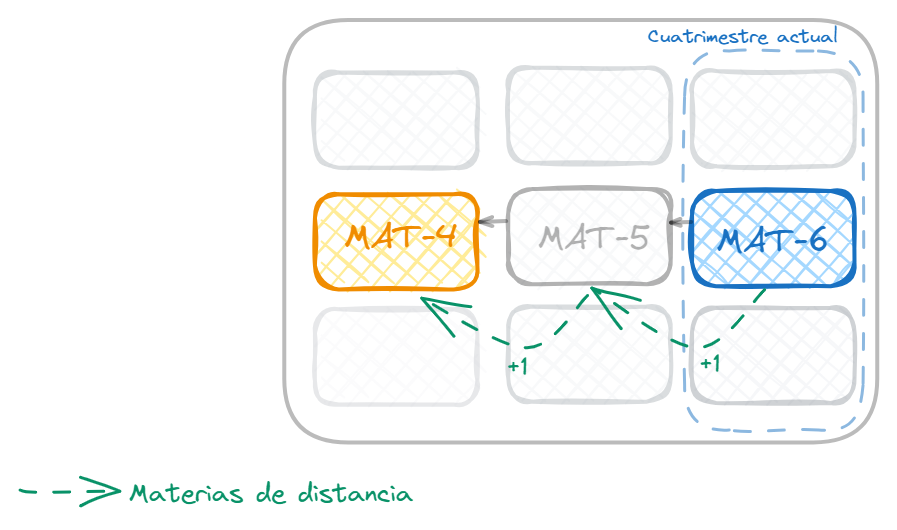
\includegraphics[width=0.9\textwidth]{images/AG-Simple-Serial-Umbral-Relevancia.png}
    \caption{Ejemplo ilustrativo de cálculo de relevancia.}
    \label{fig:ejemplo_ilustrativo_calculo_de_relevancia}
\end{figure}

Por ejemplo, consideremos el caso del umbral de la materia MAT-4 de la figura \ref{fig:ejemplo_ilustrativo_calculo_de_relevancia} para un alumno en sexto semestre. En este caso, se sumará 1 punto al umbral base de 1 debido a que MAT-4 es una materia dependiente. Además, si el último cuatrimestre actual del alumno es mayor al cuatrimestre en el que se ofrece la materia MAT-4, se añadirá un punto adicional al umbral por cada cuatrimestre de diferencia entre el último cuatrimestre actual y el cuatrimestre de la materia.

Para ilustrar el cálculo del umbral de relevancia de la materia MAT-4 para un alumno en sexto semestre, consideremos los siguientes factores:

MAT-4 comienza con un umbral de 1, que es el valor predeterminado de todas las materias. Al ser dependencia de las materias MAT-5 hasta MAT-9, lo que suma un total de 5 materias dependientes, se añade 1 punto al umbral por cada una de estas materias, lo que suma un total de 5 puntos adicionales al umbral original de 1, resultando en un umbral de 6.

Además, el alumno se encuentra en el cuatrimestre 6, mientras que la carga donde se halla la materia MAT-4 está a 2 cuatrimestres de distancia. Por cada cuatrimestre de diferencia entre el último cuatrimestre actual del alumno y el cuatrimestre de la materia, se suma un punto adicional al umbral de relevancia de la materia. Por lo tanto, se añadirán 2 puntos al umbral, lo que resulta en un umbral final de relevancia de 8 para la materia MAT-4 en este ejemplo.

Este proceso ilustra cómo se calcula el umbral de relevancia de una materia, teniendo en cuenta tanto sus dependencias como la distancia en cuatrimestres entre el último cuatrimestre actual del alumno y el cuatrimestre en el que se ofrece la materia.

\subsection{Procesamientode la información} \label{procesamiento_de_la_informacion}